\documentclass[1p]{elsarticle_modified}
%\bibliographystyle{elsarticle-num}

%\usepackage[colorlinks]{hyperref}
%\usepackage{abbrmath_seonhwa} %\Abb, \Ascr, \Acal ,\Abf, \Afrak
\usepackage{amsfonts}
\usepackage{amssymb}
\usepackage{amsmath}
\usepackage{amsthm}
\usepackage{scalefnt}
\usepackage{amsbsy}
\usepackage{kotex}
\usepackage{caption}
\usepackage{subfig}
\usepackage{color}
\usepackage{graphicx}
\usepackage{xcolor} %% white, black, red, green, blue, cyan, magenta, yellow
\usepackage{float}
\usepackage{setspace}
\usepackage{hyperref}

\usepackage{tikz}
\usetikzlibrary{arrows}

\usepackage{multirow}
\usepackage{array} % fixed length table
\usepackage{hhline}

%%%%%%%%%%%%%%%%%%%%%
\makeatletter
\renewcommand*\env@matrix[1][\arraystretch]{%
	\edef\arraystretch{#1}%
	\hskip -\arraycolsep
	\let\@ifnextchar\new@ifnextchar
	\array{*\c@MaxMatrixCols c}}
\makeatother %https://tex.stackexchange.com/questions/14071/how-can-i-increase-the-line-spacing-in-a-matrix
%%%%%%%%%%%%%%%

\usepackage[normalem]{ulem}

\newcommand{\msout}[1]{\ifmmode\text{\sout{\ensuremath{#1}}}\else\sout{#1}\fi}
%SOURCE: \msout is \stkout macro in https://tex.stackexchange.com/questions/20609/strikeout-in-math-mode

\newcommand{\cancel}[1]{
	\ifmmode
	{\color{red}\msout{#1}}
	\else
	{\color{red}\sout{#1}}
	\fi
}

\newcommand{\add}[1]{
	{\color{blue}\uwave{#1}}
}

\newcommand{\replace}[2]{
	\ifmmode
	{\color{red}\msout{#1}}{\color{blue}\uwave{#2}}
	\else
	{\color{red}\sout{#1}}{\color{blue}\uwave{#2}}
	\fi
}

\newcommand{\Sol}{\mathcal{S}} %segment
\newcommand{\D}{D} %diagram
\newcommand{\A}{\mathcal{A}} %arc


%%%%%%%%%%%%%%%%%%%%%%%%%%%%%5 test

\def\sl{\operatorname{\textup{SL}}(2,\Cbb)}
\def\psl{\operatorname{\textup{PSL}}(2,\Cbb)}
\def\quan{\mkern 1mu \triangleright \mkern 1mu}

\theoremstyle{definition}
\newtheorem{thm}{Theorem}[section]
\newtheorem{prop}[thm]{Proposition}
\newtheorem{lem}[thm]{Lemma}
\newtheorem{ques}[thm]{Question}
\newtheorem{cor}[thm]{Corollary}
\newtheorem{defn}[thm]{Definition}
\newtheorem{exam}[thm]{Example}
\newtheorem{rmk}[thm]{Remark}
\newtheorem{alg}[thm]{Algorithm}

\newcommand{\I}{\sqrt{-1}}
\begin{document}

%\begin{frontmatter}
%
%\title{Boundary parabolic representations of knots up to 8 crossings}
%
%%% Group authors per affiliation:
%\author{Yunhi Cho} 
%\address{Department of Mathematics, University of Seoul, Seoul, Korea}
%\ead{yhcho@uos.ac.kr}
%
%
%\author{Seonhwa Kim} %\fnref{s_kim}}
%\address{Center for Geometry and Physics, Institute for Basic Science, Pohang, 37673, Korea}
%\ead{ryeona17@ibs.re.kr}
%
%\author{Hyuk Kim}
%\address{Department of Mathematical Sciences, Seoul National University, Seoul 08826, Korea}
%\ead{hyukkim@snu.ac.kr}
%
%\author{Seokbeom Yoon}
%\address{Department of Mathematical Sciences, Seoul National University, Seoul, 08826,  Korea}
%\ead{sbyoon15@snu.ac.kr}
%
%\begin{abstract}
%We find all boundary parabolic representation of knots up to 8 crossings.
%
%\end{abstract}
%\begin{keyword}
%    \MSC[2010] 57M25 
%\end{keyword}
%
%\end{frontmatter}

%\linenumbers
%\tableofcontents
%
\newcommand\colored[1]{\textcolor{white}{\rule[-0.35ex]{0.8em}{1.4ex}}\kern-0.8em\color{red} #1}%
%\newcommand\colored[1]{\textcolor{white}{ #1}\kern-2.17ex	\textcolor{white}{ #1}\kern-1.81ex	\textcolor{white}{ #1}\kern-2.15ex\color{red}#1	}

{\Large $\underline{12a_{0818}~(K12a_{0818})}$}

\setlength{\tabcolsep}{10pt}
\renewcommand{\arraystretch}{1.6}
\vspace{1cm}\begin{tabular}{m{100pt}>{\centering\arraybackslash}m{274pt}}
\multirow{5}{120pt}{
	\centering
	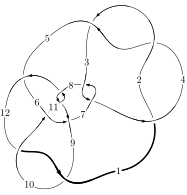
\includegraphics[width=112pt]{../../../GIT/diagram.site/Diagrams/png/1619_12a_0818.png}\\
\ \ \ A knot diagram\footnotemark}&
\allowdisplaybreaks
\textbf{Linearized knot diagam} \\
\cline{2-2}
 &
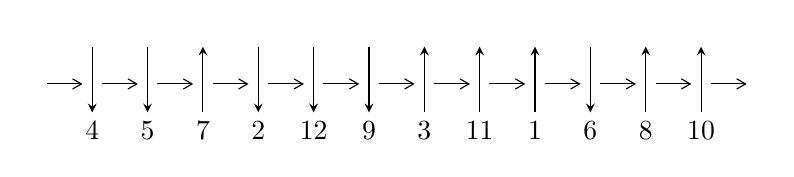
\begin{tikzpicture}[x=20pt, y=17pt]
	% nodes
	\node (C0) at (0, 0) {};
	\node (C1) at (1, 0) {};
	\node (C1U) at (1, +1) {};
	\node (C1D) at (1, -1) {4};

	\node (C2) at (2, 0) {};
	\node (C2U) at (2, +1) {};
	\node (C2D) at (2, -1) {5};

	\node (C3) at (3, 0) {};
	\node (C3U) at (3, +1) {};
	\node (C3D) at (3, -1) {7};

	\node (C4) at (4, 0) {};
	\node (C4U) at (4, +1) {};
	\node (C4D) at (4, -1) {2};

	\node (C5) at (5, 0) {};
	\node (C5U) at (5, +1) {};
	\node (C5D) at (5, -1) {12};

	\node (C6) at (6, 0) {};
	\node (C6U) at (6, +1) {};
	\node (C6D) at (6, -1) {9};

	\node (C7) at (7, 0) {};
	\node (C7U) at (7, +1) {};
	\node (C7D) at (7, -1) {3};

	\node (C8) at (8, 0) {};
	\node (C8U) at (8, +1) {};
	\node (C8D) at (8, -1) {11};

	\node (C9) at (9, 0) {};
	\node (C9U) at (9, +1) {};
	\node (C9D) at (9, -1) {1};

	\node (C10) at (10, 0) {};
	\node (C10U) at (10, +1) {};
	\node (C10D) at (10, -1) {6};

	\node (C11) at (11, 0) {};
	\node (C11U) at (11, +1) {};
	\node (C11D) at (11, -1) {8};

	\node (C12) at (12, 0) {};
	\node (C12U) at (12, +1) {};
	\node (C12D) at (12, -1) {10};
	\node (C13) at (13, 0) {};

	% arrows
	\draw[->,>={angle 60}]
	(C0) edge (C1) (C1) edge (C2) (C2) edge (C3) (C3) edge (C4) (C4) edge (C5) (C5) edge (C6) (C6) edge (C7) (C7) edge (C8) (C8) edge (C9) (C9) edge (C10) (C10) edge (C11) (C11) edge (C12) (C12) edge (C13) ;	\draw[->,>=stealth]
	(C1U) edge (C1D) (C2U) edge (C2D) (C3D) edge (C3U) (C4U) edge (C4D) (C5U) edge (C5D) (C6U) edge (C6D) (C7D) edge (C7U) (C8D) edge (C8U) (C9D) edge (C9U) (C10U) edge (C10D) (C11D) edge (C11U) (C12D) edge (C12U) ;
	\end{tikzpicture} \\
\hhline{~~} \\& 
\textbf{Solving Sequence} \\ \cline{2-2} 
 &
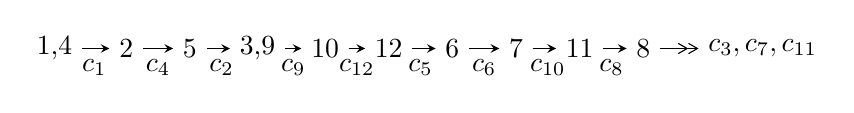
\begin{tikzpicture}[x=23pt, y=7pt]
	% node
	\node (A0) at (-1/8, 0) {1,4};
	\node (A1) at (1, 0) {2};
	\node (A2) at (2, 0) {5};
	\node (A3) at (49/16, 0) {3,9};
	\node (A4) at (33/8, 0) {10};
	\node (A5) at (41/8, 0) {12};
	\node (A6) at (49/8, 0) {6};
	\node (A7) at (57/8, 0) {7};
	\node (A8) at (65/8, 0) {11};
	\node (A9) at (73/8, 0) {8};
	\node (C1) at (1/2, -1) {$c_{1}$};
	\node (C2) at (3/2, -1) {$c_{4}$};
	\node (C3) at (5/2, -1) {$c_{2}$};
	\node (C4) at (29/8, -1) {$c_{9}$};
	\node (C5) at (37/8, -1) {$c_{12}$};
	\node (C6) at (45/8, -1) {$c_{5}$};
	\node (C7) at (53/8, -1) {$c_{6}$};
	\node (C8) at (61/8, -1) {$c_{10}$};
	\node (C9) at (69/8, -1) {$c_{8}$};
	\node (A10) at (11, 0) {$c_{3},c_{7},c_{11}$};

	% edge
	\draw[->,>=stealth]	
	(A0) edge (A1) (A1) edge (A2) (A2) edge (A3) (A3) edge (A4) (A4) edge (A5) (A5) edge (A6) (A6) edge (A7) (A7) edge (A8) (A8) edge (A9) ;
	\draw[->>,>={angle 60}]	
	(A9) edge (A10);
\end{tikzpicture} \\ 

\end{tabular} \\

\footnotetext{
The image of knot diagram is generated by the software ``\textbf{Draw programme}" developed by Andrew Bartholomew(\url{http://www.layer8.co.uk/maths/draw/index.htm\#Running-draw}), where we modified some parts for our purpose(\url{https://github.com/CATsTAILs/LinksPainter}).
}\phantom \\ \newline 
\centering \textbf{Ideals for irreducible components\footnotemark of $X_{\text{par}}$} 
 
\begin{align*}
I^u_{1}&=\langle 
4.70557\times10^{47} u^{41}+1.02379\times10^{48} u^{40}+\cdots+2.35995\times10^{48} b-1.46322\times10^{48},\\
\phantom{I^u_{1}}&\phantom{= \langle  }-2.68217\times10^{48} u^{41}-8.92209\times10^{48} u^{40}+\cdots+6.29321\times10^{48} a-9.88859\times10^{49},\\
\phantom{I^u_{1}}&\phantom{= \langle  }u^{42}+4 u^{41}+\cdots+65 u+16\rangle \\
I^u_{2}&=\langle 
431 u^{34} a-1267 u^{34}+\cdots+287 a-903,\;-3 u^{34} a+24 u^{34}+\cdots+3 a+14,\;u^{35}+4 u^{34}+\cdots+3 u+1\rangle \\
I^u_{3}&=\langle 
16 a^3+b+3 a-6,\;4 a^4-3 a^3+a^2-2 a+1,\;u-1\rangle \\
I^u_{4}&=\langle 
b-1,\;-2 u^3-2 u^2+2 a+2 u+3,\;u^5+u^4-2 u^3- u^2+u-1\rangle \\
I^u_{5}&=\langle 
- a^5+2 a^4+8 a^3-27 a^2+11 b+20 a+4,\;a^6-5 a^5+9 a^4-4 a^3-2 a^2+a+1,\;u-1\rangle \\
\\
\end{align*}
\raggedright * 5 irreducible components of $\dim_{\mathbb{C}}=0$, with total 127 representations.\\
\footnotetext{All coefficients of polynomials are rational numbers. But the coefficients are sometimes approximated in decimal forms when there is not enough margin.}
\newpage
\renewcommand{\arraystretch}{1}
\centering \section*{I. $I^u_{1}= \langle 4.71\times10^{47} u^{41}+1.02\times10^{48} u^{40}+\cdots+2.36\times10^{48} b-1.46\times10^{48},\;-2.68\times10^{48} u^{41}-8.92\times10^{48} u^{40}+\cdots+6.29\times10^{48} a-9.89\times10^{49},\;u^{42}+4 u^{41}+\cdots+65 u+16 \rangle$}
\flushleft \textbf{(i) Arc colorings}\\
\begin{tabular}{m{7pt} m{180pt} m{7pt} m{180pt} }
\flushright $a_{1}=$&$\begin{pmatrix}1\\0\end{pmatrix}$ \\
\flushright $a_{4}=$&$\begin{pmatrix}0\\u\end{pmatrix}$ \\
\flushright $a_{2}=$&$\begin{pmatrix}1\\u^2\end{pmatrix}$ \\
\flushright $a_{5}=$&$\begin{pmatrix}- u\\- u^3+u\end{pmatrix}$ \\
\flushright $a_{3}=$&$\begin{pmatrix}- u^2+1\\- u^4+2 u^2\end{pmatrix}$ \\
\flushright $a_{9}=$&$\begin{pmatrix}0.426201 u^{41}+1.41773 u^{40}+\cdots+26.1957 u+15.7131\\-0.199393 u^{41}-0.433818 u^{40}+\cdots-8.03052 u+0.620022\end{pmatrix}$ \\
\flushright $a_{10}=$&$\begin{pmatrix}0.226808 u^{41}+0.983916 u^{40}+\cdots+18.1651 u+16.3331\\-0.199393 u^{41}-0.433818 u^{40}+\cdots-8.03052 u+0.620022\end{pmatrix}$ \\
\flushright $a_{12}=$&$\begin{pmatrix}-0.130478 u^{41}-0.589048 u^{40}+\cdots-7.93921 u-10.8045\\0.214517 u^{41}+0.476122 u^{40}+\cdots+8.74596 u-0.0471007\end{pmatrix}$ \\
\flushright $a_{6}=$&$\begin{pmatrix}0.00615099 u^{41}+0.0315685 u^{40}+\cdots+2.33674 u+0.767602\\0.0725771 u^{41}+0.173370 u^{40}+\cdots+2.50038 u+1.45174\end{pmatrix}$ \\
\flushright $a_{7}=$&$\begin{pmatrix}-0.213738 u^{41}-0.514758 u^{40}+\cdots-2.95723 u-3.48358\\0.0448717 u^{41}-0.0100936 u^{40}+\cdots-0.439227 u-0.620256\end{pmatrix}$ \\
\flushright $a_{11}=$&$\begin{pmatrix}0.382659 u^{41}+1.46025 u^{40}+\cdots+24.9207 u+21.9393\\0.0557291 u^{41}+0.360679 u^{40}+\cdots+2.82601 u+7.24218\end{pmatrix}$ \\
\flushright $a_{8}=$&$\begin{pmatrix}0.111846 u^{41}+0.317186 u^{40}+\cdots+11.7593 u+0.621293\\0.0138015 u^{41}-0.0198181 u^{40}+\cdots-0.199133 u-0.618692\end{pmatrix}$\\&\end{tabular}
\flushleft \textbf{(ii) Obstruction class $= -1$}\\~\\
\flushleft \textbf{(iii) Cusp Shapes $= 1.14636 u^{41}+3.75809 u^{40}+\cdots+70.7450 u+50.8762$}\\~\\
\newpage\renewcommand{\arraystretch}{1}
\flushleft \textbf{(iv) u-Polynomials at the component}\newline \\
\begin{tabular}{m{50pt}|m{274pt}}
Crossings & \hspace{64pt}u-Polynomials at each crossing \\
\hline $$\begin{aligned}c_{1},c_{2},c_{4}\end{aligned}$$&$\begin{aligned}
&u^{42}-4 u^{41}+\cdots-65 u+16
\end{aligned}$\\
\hline $$\begin{aligned}c_{3},c_{7}\end{aligned}$$&$\begin{aligned}
&u^{42}+12 u^{40}+\cdots+800 u-256
\end{aligned}$\\
\hline $$\begin{aligned}c_{5},c_{6}\end{aligned}$$&$\begin{aligned}
&32(32 u^{42}-80 u^{41}+\cdots-4 u^2+1)
\end{aligned}$\\
\hline $$\begin{aligned}c_{8},c_{9},c_{11}\\c_{12}\end{aligned}$$&$\begin{aligned}
&u^{42}-5 u^{41}+\cdots-9 u-1
\end{aligned}$\\
\hline $$\begin{aligned}c_{10}\end{aligned}$$&$\begin{aligned}
&u^{42}+6 u^{41}+\cdots+23552 u+4096
\end{aligned}$\\
\hline
\end{tabular}\\~\\
\newpage\renewcommand{\arraystretch}{1}
\flushleft \textbf{(v) Riley Polynomials at the component}\newline \\
\begin{tabular}{m{50pt}|m{274pt}}
Crossings & \hspace{64pt}Riley Polynomials at each crossing \\
\hline $$\begin{aligned}c_{1},c_{2},c_{4}\end{aligned}$$&$\begin{aligned}
&y^{42}-40 y^{41}+\cdots-2401 y+256
\end{aligned}$\\
\hline $$\begin{aligned}c_{3},c_{7}\end{aligned}$$&$\begin{aligned}
&y^{42}+24 y^{41}+\cdots-54272 y+65536
\end{aligned}$\\
\hline $$\begin{aligned}c_{5},c_{6}\end{aligned}$$&$\begin{aligned}
&1024(1024 y^{42}-12544 y^{41}+\cdots-8 y+1)
\end{aligned}$\\
\hline $$\begin{aligned}c_{8},c_{9},c_{11}\\c_{12}\end{aligned}$$&$\begin{aligned}
&y^{42}+21 y^{41}+\cdots-57 y+1
\end{aligned}$\\
\hline $$\begin{aligned}c_{10}\end{aligned}$$&$\begin{aligned}
&y^{42}-12 y^{41}+\cdots-370147328 y+16777216
\end{aligned}$\\
\hline
\end{tabular}\\~\\
\newpage\flushleft \textbf{(vi) Complex Volumes and Cusp Shapes}
$$\begin{array}{c|c|c}  
\text{Solutions to }I^u_{1}& \I (\text{vol} + \sqrt{-1}CS) & \text{Cusp shape}\\
 \hline 
\begin{aligned}
u &= \phantom{-}0.382277 + 0.955337 I \\
a &= -1.66113 + 0.73518 I \\
b &= \phantom{-}0.53625 - 1.35310 I\end{aligned}
 & -7.2700 - 13.9728 I & -5.21740 + 8.75518 I \\ \hline\begin{aligned}
u &= \phantom{-}0.382277 - 0.955337 I \\
a &= -1.66113 - 0.73518 I \\
b &= \phantom{-}0.53625 + 1.35310 I\end{aligned}
 & -7.2700 + 13.9728 I & -5.21740 - 8.75518 I \\ \hline\begin{aligned}
u &= \phantom{-}1.036130 + 0.136384 I \\
a &= \phantom{-}0.31397 + 1.71197 I \\
b &= -0.698855 + 0.209140 I\end{aligned}
 & -0.378272 - 0.672845 I & \phantom{-}8.32593 - 8.18018 I \\ \hline\begin{aligned}
u &= \phantom{-}1.036130 - 0.136384 I \\
a &= \phantom{-}0.31397 - 1.71197 I \\
b &= -0.698855 - 0.209140 I\end{aligned}
 & -0.378272 + 0.672845 I & \phantom{-}8.32593 + 8.18018 I \\ \hline\begin{aligned}
u &= -0.176431 + 0.920219 I \\
a &= -0.089233 + 0.806500 I \\
b &= \phantom{-}0.260719 - 1.022000 I\end{aligned}
 & -1.94168 - 4.58363 I & -2.67478 + 9.67087 I \\ \hline\begin{aligned}
u &= -0.176431 - 0.920219 I \\
a &= -0.089233 - 0.806500 I \\
b &= \phantom{-}0.260719 + 1.022000 I\end{aligned}
 & -1.94168 + 4.58363 I & -2.67478 - 9.67087 I \\ \hline\begin{aligned}
u &= \phantom{-}1.16532\phantom{ +0.000000I} \\
a &= -0.690948\phantom{ +0.000000I} \\
b &= \phantom{-}0.111472\phantom{ +0.000000I}\end{aligned}
 & -2.22469\phantom{ +0.000000I} & -4.45330\phantom{ +0.000000I} \\ \hline\begin{aligned}
u &= \phantom{-}0.906961 + 0.760300 I \\
a &= -0.164799 - 0.716064 I \\
b &= \phantom{-}0.451974 + 1.333990 I\end{aligned}
 & -8.82177 + 8.14344 I & -7.68661 - 4.52240 I \\ \hline\begin{aligned}
u &= \phantom{-}0.906961 - 0.760300 I \\
a &= -0.164799 + 0.716064 I \\
b &= \phantom{-}0.451974 - 1.333990 I\end{aligned}
 & -8.82177 - 8.14344 I & -7.68661 + 4.52240 I \\ \hline\begin{aligned}
u &= -1.201200 + 0.145400 I \\
a &= -0.872305 - 0.102731 I \\
b &= \phantom{-}0.574673 + 1.022490 I\end{aligned}
 & -4.65035 + 8.25878 I & -8.8821 - 11.5403 I\\
 \hline 
 \end{array}$$\newpage$$\begin{array}{c|c|c}  
\text{Solutions to }I^u_{1}& \I (\text{vol} + \sqrt{-1}CS) & \text{Cusp shape}\\
 \hline 
\begin{aligned}
u &= -1.201200 - 0.145400 I \\
a &= -0.872305 + 0.102731 I \\
b &= \phantom{-}0.574673 - 1.022490 I\end{aligned}
 & -4.65035 - 8.25878 I & -8.8821 + 11.5403 I \\ \hline\begin{aligned}
u &= \phantom{-}0.518201 + 1.133520 I \\
a &= \phantom{-}0.589570 - 0.397152 I \\
b &= -0.152757 + 1.101360 I\end{aligned}
 & -4.92726 - 4.44307 I & -10.0669 + 11.2674 I \\ \hline\begin{aligned}
u &= \phantom{-}0.518201 - 1.133520 I \\
a &= \phantom{-}0.589570 + 0.397152 I \\
b &= -0.152757 - 1.101360 I\end{aligned}
 & -4.92726 + 4.44307 I & -10.0669 - 11.2674 I \\ \hline\begin{aligned}
u &= \phantom{-}0.391460 + 0.629294 I \\
a &= \phantom{-}2.37670 + 0.71559 I \\
b &= -1.257320 - 0.163098 I\end{aligned}
 & \phantom{-}1.03974 - 1.89674 I & -9.71636 + 10.18048 I \\ \hline\begin{aligned}
u &= \phantom{-}0.391460 - 0.629294 I \\
a &= \phantom{-}2.37670 - 0.71559 I \\
b &= -1.257320 + 0.163098 I\end{aligned}
 & \phantom{-}1.03974 + 1.89674 I & -9.71636 - 10.18048 I \\ \hline\begin{aligned}
u &= \phantom{-}1.28899\phantom{ +0.000000I} \\
a &= -0.386397\phantom{ +0.000000I} \\
b &= -1.24413\phantom{ +0.000000I}\end{aligned}
 & -1.06374\phantom{ +0.000000I} & -15.9330\phantom{ +0.000000I} \\ \hline\begin{aligned}
u &= -0.520433 + 0.480903 I \\
a &= -1.54139 + 0.22846 I \\
b &= \phantom{-}0.486493 + 1.206120 I\end{aligned}
 & -3.67601 + 8.64693 I & -1.18407 - 7.85838 I \\ \hline\begin{aligned}
u &= -0.520433 - 0.480903 I \\
a &= -1.54139 - 0.22846 I \\
b &= \phantom{-}0.486493 - 1.206120 I\end{aligned}
 & -3.67601 - 8.64693 I & -1.18407 + 7.85838 I \\ \hline\begin{aligned}
u &= -1.369360 + 0.103398 I \\
a &= \phantom{-}1.140050 - 0.314674 I \\
b &= -1.010040 - 0.754348 I\end{aligned}
 & -2.55620 + 3.08969 I & \phantom{-0.000000 } 0 \\ \hline\begin{aligned}
u &= -1.369360 - 0.103398 I \\
a &= \phantom{-}1.140050 + 0.314674 I \\
b &= -1.010040 + 0.754348 I\end{aligned}
 & -2.55620 - 3.08969 I & \phantom{-0.000000 } 0\\
 \hline 
 \end{array}$$\newpage$$\begin{array}{c|c|c}  
\text{Solutions to }I^u_{1}& \I (\text{vol} + \sqrt{-1}CS) & \text{Cusp shape}\\
 \hline 
\begin{aligned}
u &= -1.381130 + 0.223245 I \\
a &= -0.587328 + 0.140475 I \\
b &= \phantom{-}0.398228 - 0.245218 I\end{aligned}
 & -5.21752 + 3.92091 I & \phantom{-0.000000 } 0 \\ \hline\begin{aligned}
u &= -1.381130 - 0.223245 I \\
a &= -0.587328 - 0.140475 I \\
b &= \phantom{-}0.398228 + 0.245218 I\end{aligned}
 & -5.21752 - 3.92091 I & \phantom{-0.000000 } 0 \\ \hline\begin{aligned}
u &= -1.46546 + 0.23954 I \\
a &= \phantom{-}0.778883 - 0.741783 I \\
b &= -1.44538 + 0.24251 I\end{aligned}
 & -4.97209 + 5.11669 I & \phantom{-0.000000 } 0 \\ \hline\begin{aligned}
u &= -1.46546 - 0.23954 I \\
a &= \phantom{-}0.778883 + 0.741783 I \\
b &= -1.44538 - 0.24251 I\end{aligned}
 & -4.97209 - 5.11669 I & \phantom{-0.000000 } 0 \\ \hline\begin{aligned}
u &= \phantom{-}1.22748 + 0.83655 I \\
a &= -0.546316 + 0.174607 I \\
b &= \phantom{-}0.091410 - 1.130240 I\end{aligned}
 & -6.99380 - 2.96639 I & \phantom{-0.000000 } 0 \\ \hline\begin{aligned}
u &= \phantom{-}1.22748 - 0.83655 I \\
a &= -0.546316 - 0.174607 I \\
b &= \phantom{-}0.091410 + 1.130240 I\end{aligned}
 & -6.99380 + 2.96639 I & \phantom{-0.000000 } 0 \\ \hline\begin{aligned}
u &= \phantom{-}0.208756 + 0.468070 I \\
a &= -1.034920 - 0.197444 I \\
b &= \phantom{-}0.106914 + 0.216906 I\end{aligned}
 & -0.189441 - 1.194630 I & -3.03902 + 4.48079 I \\ \hline\begin{aligned}
u &= \phantom{-}0.208756 - 0.468070 I \\
a &= -1.034920 + 0.197444 I \\
b &= \phantom{-}0.106914 - 0.216906 I\end{aligned}
 & -0.189441 + 1.194630 I & -3.03902 - 4.48079 I \\ \hline\begin{aligned}
u &= \phantom{-}1.49536 + 0.19812 I \\
a &= -1.070210 - 0.916497 I \\
b &= \phantom{-}0.49427 - 1.35780 I\end{aligned}
 & -10.2159 - 11.2963 I & \phantom{-0.000000 } 0 \\ \hline\begin{aligned}
u &= \phantom{-}1.49536 - 0.19812 I \\
a &= -1.070210 + 0.916497 I \\
b &= \phantom{-}0.49427 + 1.35780 I\end{aligned}
 & -10.2159 + 11.2963 I & \phantom{-0.000000 } 0\\
 \hline 
 \end{array}$$\newpage$$\begin{array}{c|c|c}  
\text{Solutions to }I^u_{1}& \I (\text{vol} + \sqrt{-1}CS) & \text{Cusp shape}\\
 \hline 
\begin{aligned}
u &= -1.50308 + 0.37191 I \\
a &= -1.59621 + 0.46175 I \\
b &= \phantom{-}0.59118 + 1.39047 I\end{aligned}
 & -13.3178 + 18.7741 I & \phantom{-0.000000 } 0 \\ \hline\begin{aligned}
u &= -1.50308 - 0.37191 I \\
a &= -1.59621 - 0.46175 I \\
b &= \phantom{-}0.59118 - 1.39047 I\end{aligned}
 & -13.3178 - 18.7741 I & \phantom{-0.000000 } 0 \\ \hline\begin{aligned}
u &= \phantom{-}0.103524 + 0.426968 I \\
a &= \phantom{-}2.10169 - 1.36256 I \\
b &= -0.922128 + 0.404344 I\end{aligned}
 & \phantom{-}2.10350 - 1.31837 I & \phantom{-}6.89891 - 1.71793 I \\ \hline\begin{aligned}
u &= \phantom{-}0.103524 - 0.426968 I \\
a &= \phantom{-}2.10169 + 1.36256 I \\
b &= -0.922128 - 0.404344 I\end{aligned}
 & \phantom{-}2.10350 + 1.31837 I & \phantom{-}6.89891 + 1.71793 I \\ \hline\begin{aligned}
u &= -1.56428 + 0.38662 I \\
a &= \phantom{-}0.947107 - 0.401179 I \\
b &= -0.300179 - 1.217090 I\end{aligned}
 & -11.6070 + 9.8095 I & \phantom{-0.000000 } 0 \\ \hline\begin{aligned}
u &= -1.56428 - 0.38662 I \\
a &= \phantom{-}0.947107 + 0.401179 I \\
b &= -0.300179 + 1.217090 I\end{aligned}
 & -11.6070 - 9.8095 I & \phantom{-0.000000 } 0 \\ \hline\begin{aligned}
u &= -0.333406 + 0.020280 I \\
a &= -0.65169 + 1.58358 I \\
b &= -0.387814 + 0.633347 I\end{aligned}
 & \phantom{-}0.54776 - 1.46692 I & \phantom{-}5.66103 + 4.76123 I \\ \hline\begin{aligned}
u &= -0.333406 - 0.020280 I \\
a &= -0.65169 - 1.58358 I \\
b &= -0.387814 - 0.633347 I\end{aligned}
 & \phantom{-}0.54776 + 1.46692 I & \phantom{-}5.66103 - 4.76123 I \\ \hline\begin{aligned}
u &= -1.67473 + 0.04568 I \\
a &= -0.132515 - 0.361034 I \\
b &= \phantom{-}0.27984 - 1.41003 I\end{aligned}
 & -18.2575 - 5.2882 I & \phantom{-0.000000 } 0 \\ \hline\begin{aligned}
u &= -1.67473 - 0.04568 I \\
a &= -0.132515 + 0.361034 I \\
b &= \phantom{-}0.27984 + 1.41003 I\end{aligned}
 & -18.2575 + 5.2882 I & \phantom{-0.000000 } 0\\
 \hline 
 \end{array}$$\newpage$$\begin{array}{c|c|c}  
\text{Solutions to }I^u_{1}& \I (\text{vol} + \sqrt{-1}CS) & \text{Cusp shape}\\
 \hline 
\begin{aligned}
u &= \phantom{-}1.69220 + 0.30592 I \\
a &= \phantom{-}0.394986 + 0.353146 I \\
b &= -0.031137 + 1.135330 I\end{aligned}
 & -8.08716 - 1.02616 I & \phantom{-0.000000 } 0 \\ \hline\begin{aligned}
u &= \phantom{-}1.69220 - 0.30592 I \\
a &= \phantom{-}0.394986 - 0.353146 I \\
b &= -0.031137 - 1.135330 I\end{aligned}
 & -8.08716 + 1.02616 I & \phantom{-0.000000 } 0\\
 \hline 
 \end{array}$$\newpage\newpage\renewcommand{\arraystretch}{1}
\centering \section*{II. $I^u_{2}= \langle 431 u^{34} a-1267 u^{34}+\cdots+287 a-903,\;-3 u^{34} a+24 u^{34}+\cdots+3 a+14,\;u^{35}+4 u^{34}+\cdots+3 u+1 \rangle$}
\flushleft \textbf{(i) Arc colorings}\\
\begin{tabular}{m{7pt} m{180pt} m{7pt} m{180pt} }
\flushright $a_{1}=$&$\begin{pmatrix}1\\0\end{pmatrix}$ \\
\flushright $a_{4}=$&$\begin{pmatrix}0\\u\end{pmatrix}$ \\
\flushright $a_{2}=$&$\begin{pmatrix}1\\u^2\end{pmatrix}$ \\
\flushright $a_{5}=$&$\begin{pmatrix}- u\\- u^3+u\end{pmatrix}$ \\
\flushright $a_{3}=$&$\begin{pmatrix}- u^2+1\\- u^4+2 u^2\end{pmatrix}$ \\
\flushright $a_{9}=$&$\begin{pmatrix}a\\-2.59639 a u^{34}+7.63253 u^{34}+\cdots-1.72892 a+5.43976\end{pmatrix}$ \\
\flushright $a_{10}=$&$\begin{pmatrix}-2.59639 a u^{34}+7.63253 u^{34}+\cdots-0.728916 a+5.43976\\-2.59639 a u^{34}+7.63253 u^{34}+\cdots-1.72892 a+5.43976\end{pmatrix}$ \\
\flushright $a_{12}=$&$\begin{pmatrix}-6.19880 a u^{34}-4.53916 u^{34}+\cdots-3.90964 a-4.43675\\-6.31627 a u^{34}-2.84639 u^{34}+\cdots-4.71988 a-2.97892\end{pmatrix}$ \\
\flushright $a_{6}=$&$\begin{pmatrix}6.56325 a u^{34}-15.4307 u^{34}+\cdots+2.74398 a-3.80422\\-0.0391566 a u^{34}-6.60241 u^{34}+\cdots+0.0632530 a-2.68072\end{pmatrix}$ \\
\flushright $a_{7}=$&$\begin{pmatrix}-\frac{7}{2} u^{34}-\frac{17}{2} u^{33}+\cdots-9 u-\frac{3}{2}\\\frac{21}{4} u^{34}+\frac{57}{4} u^{33}+\cdots+9 u+\frac{19}{4}\end{pmatrix}$ \\
\flushright $a_{11}=$&$\begin{pmatrix}7.63253 a u^{34}+1.94277 u^{34}+\cdots+5.43976 a+2.70783\\1\end{pmatrix}$ \\
\flushright $a_{8}=$&$\begin{pmatrix}\frac{7}{2} u^{34}+\frac{19}{2} u^{33}+\cdots+2 u+\frac{7}{2}\\\frac{31}{4} u^{34}+\frac{83}{4} u^{33}+\cdots+12 u+\frac{25}{4}\end{pmatrix}$\\&\end{tabular}
\flushleft \textbf{(ii) Obstruction class $= -1$}\\~\\
\flushleft \textbf{(iii) Cusp Shapes $= 10 u^{34}+\frac{55}{2} u^{33}+\cdots+\frac{39}{2} u+\frac{13}{2}$}\\~\\
\newpage\renewcommand{\arraystretch}{1}
\flushleft \textbf{(iv) u-Polynomials at the component}\newline \\
\begin{tabular}{m{50pt}|m{274pt}}
Crossings & \hspace{64pt}u-Polynomials at each crossing \\
\hline $$\begin{aligned}c_{1},c_{2},c_{4}\end{aligned}$$&$\begin{aligned}
&(u^{35}-4 u^{34}+\cdots+3 u-1)^{2}
\end{aligned}$\\
\hline $$\begin{aligned}c_{3},c_{7}\end{aligned}$$&$\begin{aligned}
&(u^{35}- u^{34}+\cdots-28 u-8)^{2}
\end{aligned}$\\
\hline $$\begin{aligned}c_{5},c_{6}\end{aligned}$$&$\begin{aligned}
&u^{70}-2 u^{69}+\cdots-215264236 u+17305121
\end{aligned}$\\
\hline $$\begin{aligned}c_{8},c_{9},c_{11}\\c_{12}\end{aligned}$$&$\begin{aligned}
&u^{70}+12 u^{69}+\cdots+4 u+1
\end{aligned}$\\
\hline $$\begin{aligned}c_{10}\end{aligned}$$&$\begin{aligned}
&(u^{35}-2 u^{34}+\cdots-2 u+1)^{2}
\end{aligned}$\\
\hline
\end{tabular}\\~\\
\newpage\renewcommand{\arraystretch}{1}
\flushleft \textbf{(v) Riley Polynomials at the component}\newline \\
\begin{tabular}{m{50pt}|m{274pt}}
Crossings & \hspace{64pt}Riley Polynomials at each crossing \\
\hline $$\begin{aligned}c_{1},c_{2},c_{4}\end{aligned}$$&$\begin{aligned}
&(y^{35}-34 y^{34}+\cdots+19 y-1)^{2}
\end{aligned}$\\
\hline $$\begin{aligned}c_{3},c_{7}\end{aligned}$$&$\begin{aligned}
&(y^{35}+21 y^{34}+\cdots+16 y-64)^{2}
\end{aligned}$\\
\hline $$\begin{aligned}c_{5},c_{6}\end{aligned}$$&$\begin{aligned}
&y^{70}-34 y^{69}+\cdots-9709459310743048 y+299467212824641
\end{aligned}$\\
\hline $$\begin{aligned}c_{8},c_{9},c_{11}\\c_{12}\end{aligned}$$&$\begin{aligned}
&y^{70}+46 y^{69}+\cdots+60 y^2+1
\end{aligned}$\\
\hline $$\begin{aligned}c_{10}\end{aligned}$$&$\begin{aligned}
&(y^{35}-12 y^{34}+\cdots+10 y-1)^{2}
\end{aligned}$\\
\hline
\end{tabular}\\~\\
\newpage\flushleft \textbf{(vi) Complex Volumes and Cusp Shapes}
$$\begin{array}{c|c|c}  
\text{Solutions to }I^u_{2}& \I (\text{vol} + \sqrt{-1}CS) & \text{Cusp shape}\\
 \hline 
\begin{aligned}
u &= \phantom{-}0.787288 + 0.599387 I \\
a &= -0.086494 + 0.987313 I \\
b &= -0.409191 - 1.343070 I\end{aligned}
 & -4.38053 + 3.19486 I & -5.71319 - 2.77080 I \\ \hline\begin{aligned}
u &= \phantom{-}0.787288 + 0.599387 I \\
a &= -1.38411 - 1.00877 I \\
b &= \phantom{-}0.940264 + 0.111257 I\end{aligned}
 & -4.38053 + 3.19486 I & -5.71319 - 2.77080 I \\ \hline\begin{aligned}
u &= \phantom{-}0.787288 - 0.599387 I \\
a &= -0.086494 - 0.987313 I \\
b &= -0.409191 + 1.343070 I\end{aligned}
 & -4.38053 - 3.19486 I & -5.71319 + 2.77080 I \\ \hline\begin{aligned}
u &= \phantom{-}0.787288 - 0.599387 I \\
a &= -1.38411 + 1.00877 I \\
b &= \phantom{-}0.940264 - 0.111257 I\end{aligned}
 & -4.38053 - 3.19486 I & -5.71319 + 2.77080 I \\ \hline\begin{aligned}
u &= \phantom{-}0.863463 + 0.435553 I \\
a &= \phantom{-}0.206812 - 0.579701 I \\
b &= -0.094077 + 1.102490 I\end{aligned}
 & -3.64066 - 1.76625 I & -4.73044 + 2.55261 I \\ \hline\begin{aligned}
u &= \phantom{-}0.863463 + 0.435553 I \\
a &= -0.608026 + 1.260340 I \\
b &= \phantom{-}0.255940 - 0.178870 I\end{aligned}
 & -3.64066 - 1.76625 I & -4.73044 + 2.55261 I \\ \hline\begin{aligned}
u &= \phantom{-}0.863463 - 0.435553 I \\
a &= \phantom{-}0.206812 + 0.579701 I \\
b &= -0.094077 - 1.102490 I\end{aligned}
 & -3.64066 + 1.76625 I & -4.73044 - 2.55261 I \\ \hline\begin{aligned}
u &= \phantom{-}0.863463 - 0.435553 I \\
a &= -0.608026 - 1.260340 I \\
b &= \phantom{-}0.255940 + 0.178870 I\end{aligned}
 & -3.64066 + 1.76625 I & -4.73044 - 2.55261 I \\ \hline\begin{aligned}
u &= \phantom{-}0.378284 + 0.838154 I \\
a &= -1.85036 - 0.34075 I \\
b &= \phantom{-}1.101690 + 0.020192 I\end{aligned}
 & -3.07931 - 8.20034 I & -2.93623 + 7.67757 I \\ \hline\begin{aligned}
u &= \phantom{-}0.378284 + 0.838154 I \\
a &= \phantom{-}1.75417 - 0.92177 I \\
b &= -0.56291 + 1.37198 I\end{aligned}
 & -3.07931 - 8.20034 I & -2.93623 + 7.67757 I\\
 \hline 
 \end{array}$$\newpage$$\begin{array}{c|c|c}  
\text{Solutions to }I^u_{2}& \I (\text{vol} + \sqrt{-1}CS) & \text{Cusp shape}\\
 \hline 
\begin{aligned}
u &= \phantom{-}0.378284 - 0.838154 I \\
a &= -1.85036 + 0.34075 I \\
b &= \phantom{-}1.101690 - 0.020192 I\end{aligned}
 & -3.07931 + 8.20034 I & -2.93623 - 7.67757 I \\ \hline\begin{aligned}
u &= \phantom{-}0.378284 - 0.838154 I \\
a &= \phantom{-}1.75417 + 0.92177 I \\
b &= -0.56291 - 1.37198 I\end{aligned}
 & -3.07931 + 8.20034 I & -2.93623 - 7.67757 I \\ \hline\begin{aligned}
u &= \phantom{-}0.535823 + 0.722828 I \\
a &= -0.45702 - 1.35557 I \\
b &= \phantom{-}0.46606 + 1.42298 I\end{aligned}
 & -7.75853 - 2.44036 I & -9.20394 + 3.90896 I \\ \hline\begin{aligned}
u &= \phantom{-}0.535823 + 0.722828 I \\
a &= -2.20201 + 0.82058 I \\
b &= \phantom{-}0.60727 - 1.30342 I\end{aligned}
 & -7.75853 - 2.44036 I & -9.20394 + 3.90896 I \\ \hline\begin{aligned}
u &= \phantom{-}0.535823 - 0.722828 I \\
a &= -0.45702 + 1.35557 I \\
b &= \phantom{-}0.46606 - 1.42298 I\end{aligned}
 & -7.75853 + 2.44036 I & -9.20394 - 3.90896 I \\ \hline\begin{aligned}
u &= \phantom{-}0.535823 - 0.722828 I \\
a &= -2.20201 - 0.82058 I \\
b &= \phantom{-}0.60727 + 1.30342 I\end{aligned}
 & -7.75853 + 2.44036 I & -9.20394 - 3.90896 I \\ \hline\begin{aligned}
u &= \phantom{-}1.11802\phantom{ +0.000000I} \\
a &= -6.86583 + 4.96782 I \\
b &= \phantom{-}0.077086 - 1.008870 I\end{aligned}
 & -5.44402\phantom{ +0.000000I} & \phantom{-}2.06430\phantom{ +0.000000I} \\ \hline\begin{aligned}
u &= \phantom{-}1.11802\phantom{ +0.000000I} \\
a &= -6.86583 - 4.96782 I \\
b &= \phantom{-}0.077086 + 1.008870 I\end{aligned}
 & -5.44402\phantom{ +0.000000I} & \phantom{-}2.06430\phantom{ +0.000000I} \\ \hline\begin{aligned}
u &= \phantom{-}0.334838 + 0.781483 I \\
a &= \phantom{-}0.611108 - 0.709436 I \\
b &= -0.266376 + 0.028486 I\end{aligned}
 & -2.04839 - 2.67684 I & -0.78426 + 2.93641 I \\ \hline\begin{aligned}
u &= \phantom{-}0.334838 + 0.781483 I \\
a &= -1.28426 + 0.62029 I \\
b &= \phantom{-}0.127641 - 1.040230 I\end{aligned}
 & -2.04839 - 2.67684 I & -0.78426 + 2.93641 I\\
 \hline 
 \end{array}$$\newpage$$\begin{array}{c|c|c}  
\text{Solutions to }I^u_{2}& \I (\text{vol} + \sqrt{-1}CS) & \text{Cusp shape}\\
 \hline 
\begin{aligned}
u &= \phantom{-}0.334838 - 0.781483 I \\
a &= \phantom{-}0.611108 + 0.709436 I \\
b &= -0.266376 - 0.028486 I\end{aligned}
 & -2.04839 + 2.67684 I & -0.78426 - 2.93641 I \\ \hline\begin{aligned}
u &= \phantom{-}0.334838 - 0.781483 I \\
a &= -1.28426 - 0.62029 I \\
b &= \phantom{-}0.127641 + 1.040230 I\end{aligned}
 & -2.04839 + 2.67684 I & -0.78426 - 2.93641 I \\ \hline\begin{aligned}
u &= -1.293330 + 0.022996 I \\
a &= -0.965695 - 0.118945 I \\
b &= \phantom{-}0.830183 - 0.558253 I\end{aligned}
 & -3.19397 + 3.04539 I & -6.49856 - 3.07346 I \\ \hline\begin{aligned}
u &= -1.293330 + 0.022996 I \\
a &= \phantom{-}0.672369 + 0.296675 I \\
b &= -0.711919 - 0.891888 I\end{aligned}
 & -3.19397 + 3.04539 I & -6.49856 - 3.07346 I \\ \hline\begin{aligned}
u &= -1.293330 - 0.022996 I \\
a &= -0.965695 + 0.118945 I \\
b &= \phantom{-}0.830183 + 0.558253 I\end{aligned}
 & -3.19397 - 3.04539 I & -6.49856 + 3.07346 I \\ \hline\begin{aligned}
u &= -1.293330 - 0.022996 I \\
a &= \phantom{-}0.672369 - 0.296675 I \\
b &= -0.711919 + 0.891888 I\end{aligned}
 & -3.19397 - 3.04539 I & -6.49856 + 3.07346 I \\ \hline\begin{aligned}
u &= \phantom{-}1.331630 + 0.151400 I \\
a &= \phantom{-}0.358567 - 0.966943 I \\
b &= -0.094807 + 0.186756 I\end{aligned}
 & -4.74191 - 0.58793 I & -2.80279 + 0. I\phantom{ +0.000000I} \\ \hline\begin{aligned}
u &= \phantom{-}1.331630 + 0.151400 I \\
a &= -1.56667 - 1.15669 I \\
b &= \phantom{-}0.033995 - 1.083710 I\end{aligned}
 & -4.74191 - 0.58793 I & -2.80279 + 0. I\phantom{ +0.000000I} \\ \hline\begin{aligned}
u &= \phantom{-}1.331630 - 0.151400 I \\
a &= \phantom{-}0.358567 + 0.966943 I \\
b &= -0.094807 - 0.186756 I\end{aligned}
 & -4.74191 + 0.58793 I & -2.80279 + 0. I\phantom{ +0.000000I} \\ \hline\begin{aligned}
u &= \phantom{-}1.331630 - 0.151400 I \\
a &= -1.56667 + 1.15669 I \\
b &= \phantom{-}0.033995 + 1.083710 I\end{aligned}
 & -4.74191 + 0.58793 I & -2.80279 + 0. I\phantom{ +0.000000I}\\
 \hline 
 \end{array}$$\newpage$$\begin{array}{c|c|c}  
\text{Solutions to }I^u_{2}& \I (\text{vol} + \sqrt{-1}CS) & \text{Cusp shape}\\
 \hline 
\begin{aligned}
u &= \phantom{-}1.40486\phantom{ +0.000000I} \\
a &= -0.474895 + 1.101280 I \\
b &= \phantom{-}0.54790 + 1.37862 I\end{aligned}
 & -9.85232\phantom{ +0.000000I} & -9.92120\phantom{ +0.000000I} \\ \hline\begin{aligned}
u &= \phantom{-}1.40486\phantom{ +0.000000I} \\
a &= -0.474895 - 1.101280 I \\
b &= \phantom{-}0.54790 - 1.37862 I\end{aligned}
 & -9.85232\phantom{ +0.000000I} & -9.92120\phantom{ +0.000000I} \\ \hline\begin{aligned}
u &= \phantom{-}1.403830 + 0.145115 I \\
a &= \phantom{-}0.98126 + 1.19495 I \\
b &= -0.49226 + 1.38247 I\end{aligned}
 & -5.78377 - 5.84473 I & \phantom{-0.000000 } 0 \\ \hline\begin{aligned}
u &= \phantom{-}1.403830 + 0.145115 I \\
a &= -0.252994 - 0.344206 I \\
b &= \phantom{-}1.053300 - 0.058898 I\end{aligned}
 & -5.78377 - 5.84473 I & \phantom{-0.000000 } 0 \\ \hline\begin{aligned}
u &= \phantom{-}1.403830 - 0.145115 I \\
a &= \phantom{-}0.98126 - 1.19495 I \\
b &= -0.49226 - 1.38247 I\end{aligned}
 & -5.78377 + 5.84473 I & \phantom{-0.000000 } 0 \\ \hline\begin{aligned}
u &= \phantom{-}1.403830 - 0.145115 I \\
a &= -0.252994 + 0.344206 I \\
b &= \phantom{-}1.053300 + 0.058898 I\end{aligned}
 & -5.78377 + 5.84473 I & \phantom{-0.000000 } 0 \\ \hline\begin{aligned}
u &= \phantom{-}0.374463 + 0.419722 I \\
a &= -2.06448 + 2.38148 I \\
b &= -0.028461 + 1.098670 I\end{aligned}
 & -3.71944 - 1.17044 I & -1.16678 + 5.64189 I \\ \hline\begin{aligned}
u &= \phantom{-}0.374463 + 0.419722 I \\
a &= \phantom{-}4.28644 + 4.59791 I \\
b &= -0.059654 - 0.866754 I\end{aligned}
 & -3.71944 - 1.17044 I & -1.16678 + 5.64189 I \\ \hline\begin{aligned}
u &= \phantom{-}0.374463 - 0.419722 I \\
a &= -2.06448 - 2.38148 I \\
b &= -0.028461 - 1.098670 I\end{aligned}
 & -3.71944 + 1.17044 I & -1.16678 - 5.64189 I \\ \hline\begin{aligned}
u &= \phantom{-}0.374463 - 0.419722 I \\
a &= \phantom{-}4.28644 - 4.59791 I \\
b &= -0.059654 + 0.866754 I\end{aligned}
 & -3.71944 + 1.17044 I & -1.16678 - 5.64189 I\\
 \hline 
 \end{array}$$\newpage$$\begin{array}{c|c|c}  
\text{Solutions to }I^u_{2}& \I (\text{vol} + \sqrt{-1}CS) & \text{Cusp shape}\\
 \hline 
\begin{aligned}
u &= -1.46236 + 0.17601 I \\
a &= \phantom{-}1.51571 - 0.46270 I \\
b &= -0.367348 + 0.819468 I\end{aligned}
 & -9.77721 + 3.48149 I & \phantom{-0.000000 } 0 \\ \hline\begin{aligned}
u &= -1.46236 + 0.17601 I \\
a &= \phantom{-}0.43467 - 1.63292 I \\
b &= -0.091480 - 1.230270 I\end{aligned}
 & -9.77721 + 3.48149 I & \phantom{-0.000000 } 0 \\ \hline\begin{aligned}
u &= -1.46236 - 0.17601 I \\
a &= \phantom{-}1.51571 + 0.46270 I \\
b &= -0.367348 - 0.819468 I\end{aligned}
 & -9.77721 - 3.48149 I & \phantom{-0.000000 } 0 \\ \hline\begin{aligned}
u &= -1.46236 - 0.17601 I \\
a &= \phantom{-}0.43467 + 1.63292 I \\
b &= -0.091480 + 1.230270 I\end{aligned}
 & -9.77721 - 3.48149 I & \phantom{-0.000000 } 0 \\ \hline\begin{aligned}
u &= -1.45963 + 0.29677 I \\
a &= \phantom{-}0.624599 + 0.193615 I \\
b &= -0.552157 - 0.070918 I\end{aligned}
 & -7.83682 + 6.58963 I & \phantom{-0.000000 } 0 \\ \hline\begin{aligned}
u &= -1.45963 + 0.29677 I \\
a &= -1.35152 + 0.58488 I \\
b &= \phantom{-}0.249550 + 1.142520 I\end{aligned}
 & -7.83682 + 6.58963 I & \phantom{-0.000000 } 0 \\ \hline\begin{aligned}
u &= -1.45963 - 0.29677 I \\
a &= \phantom{-}0.624599 - 0.193615 I \\
b &= -0.552157 + 0.070918 I\end{aligned}
 & -7.83682 - 6.58963 I & \phantom{-0.000000 } 0 \\ \hline\begin{aligned}
u &= -1.45963 - 0.29677 I \\
a &= -1.35152 - 0.58488 I \\
b &= \phantom{-}0.249550 - 1.142520 I\end{aligned}
 & -7.83682 - 6.58963 I & \phantom{-0.000000 } 0 \\ \hline\begin{aligned}
u &= -0.166758 + 0.470101 I \\
a &= -1.10634 - 1.04351 I \\
b &= -0.266545 + 0.867095 I\end{aligned}
 & -0.05478 - 1.72545 I & \phantom{-}3.36392 + 2.52233 I \\ \hline\begin{aligned}
u &= -0.166758 + 0.470101 I \\
a &= -1.20153 + 0.96877 I \\
b &= \phantom{-}0.368166 + 0.304402 I\end{aligned}
 & -0.05478 - 1.72545 I & \phantom{-}3.36392 + 2.52233 I\\
 \hline 
 \end{array}$$\newpage$$\begin{array}{c|c|c}  
\text{Solutions to }I^u_{2}& \I (\text{vol} + \sqrt{-1}CS) & \text{Cusp shape}\\
 \hline 
\begin{aligned}
u &= -0.166758 - 0.470101 I \\
a &= -1.10634 + 1.04351 I \\
b &= -0.266545 - 0.867095 I\end{aligned}
 & -0.05478 + 1.72545 I & \phantom{-}3.36392 - 2.52233 I \\ \hline\begin{aligned}
u &= -0.166758 - 0.470101 I \\
a &= -1.20153 - 0.96877 I \\
b &= \phantom{-}0.368166 - 0.304402 I\end{aligned}
 & -0.05478 + 1.72545 I & \phantom{-}3.36392 - 2.52233 I \\ \hline\begin{aligned}
u &= -0.261262 + 0.408522 I \\
a &= -0.881409 + 0.809220 I \\
b &= \phantom{-}0.850553 - 0.149091 I\end{aligned}
 & -0.43566 + 3.77887 I & \phantom{-}2.70186 - 3.89618 I \\ \hline\begin{aligned}
u &= -0.261262 + 0.408522 I \\
a &= \phantom{-}2.21730 - 0.24123 I \\
b &= -0.502121 - 1.163120 I\end{aligned}
 & -0.43566 + 3.77887 I & \phantom{-}2.70186 - 3.89618 I \\ \hline\begin{aligned}
u &= -0.261262 - 0.408522 I \\
a &= -0.881409 - 0.809220 I \\
b &= \phantom{-}0.850553 + 0.149091 I\end{aligned}
 & -0.43566 - 3.77887 I & \phantom{-}2.70186 + 3.89618 I \\ \hline\begin{aligned}
u &= -0.261262 - 0.408522 I \\
a &= \phantom{-}2.21730 + 0.24123 I \\
b &= -0.502121 + 1.163120 I\end{aligned}
 & -0.43566 - 3.77887 I & \phantom{-}2.70186 + 3.89618 I \\ \hline\begin{aligned}
u &= -1.48269 + 0.31831 I \\
a &= -0.841244 + 0.661850 I \\
b &= \phantom{-}1.235650 - 0.053997 I\end{aligned}
 & -9.0790 + 12.3988 I & \phantom{-0.000000 } 0 \\ \hline\begin{aligned}
u &= -1.48269 + 0.31831 I \\
a &= \phantom{-}1.53656 - 0.44667 I \\
b &= -0.65200 - 1.43728 I\end{aligned}
 & -9.0790 + 12.3988 I & \phantom{-0.000000 } 0 \\ \hline\begin{aligned}
u &= -1.48269 - 0.31831 I \\
a &= -0.841244 - 0.661850 I \\
b &= \phantom{-}1.235650 + 0.053997 I\end{aligned}
 & -9.0790 - 12.3988 I & \phantom{-0.000000 } 0 \\ \hline\begin{aligned}
u &= -1.48269 - 0.31831 I \\
a &= \phantom{-}1.53656 + 0.44667 I \\
b &= -0.65200 + 1.43728 I\end{aligned}
 & -9.0790 - 12.3988 I & \phantom{-0.000000 } 0\\
 \hline 
 \end{array}$$\newpage$$\begin{array}{c|c|c}  
\text{Solutions to }I^u_{2}& \I (\text{vol} + \sqrt{-1}CS) & \text{Cusp shape}\\
 \hline 
\begin{aligned}
u &= -1.52211 + 0.12323 I \\
a &= -0.684628 + 0.572571 I \\
b &= \phantom{-}1.063560 - 0.479442 I\end{aligned}
 & -12.01000 - 1.04091 I & \phantom{-0.000000 } 0 \\ \hline\begin{aligned}
u &= -1.52211 + 0.12323 I \\
a &= -0.247279 + 0.320973 I \\
b &= -0.24344 + 1.56604 I\end{aligned}
 & -12.01000 - 1.04091 I & \phantom{-0.000000 } 0 \\ \hline\begin{aligned}
u &= -1.52211 - 0.12323 I \\
a &= -0.684628 - 0.572571 I \\
b &= \phantom{-}1.063560 + 0.479442 I\end{aligned}
 & -12.01000 + 1.04091 I & \phantom{-0.000000 } 0 \\ \hline\begin{aligned}
u &= -1.52211 - 0.12323 I \\
a &= -0.247279 - 0.320973 I \\
b &= -0.24344 - 1.56604 I\end{aligned}
 & -12.01000 + 1.04091 I & \phantom{-0.000000 } 0 \\ \hline\begin{aligned}
u &= -1.51902 + 0.23855 I \\
a &= -1.50135 + 0.36894 I \\
b &= \phantom{-}0.78842 + 1.32634 I\end{aligned}
 & -14.4705 + 5.9201 I & \phantom{-0.000000 } 0 \\ \hline\begin{aligned}
u &= -1.51902 + 0.23855 I \\
a &= \phantom{-}0.181610 + 0.009514 I \\
b &= \phantom{-}0.45096 - 1.59114 I\end{aligned}
 & -14.4705 + 5.9201 I & \phantom{-0.000000 } 0 \\ \hline\begin{aligned}
u &= -1.51902 - 0.23855 I \\
a &= -1.50135 - 0.36894 I \\
b &= \phantom{-}0.78842 - 1.32634 I\end{aligned}
 & -14.4705 - 5.9201 I & \phantom{-0.000000 } 0 \\ \hline\begin{aligned}
u &= -1.51902 - 0.23855 I \\
a &= \phantom{-}0.181610 - 0.009514 I \\
b &= \phantom{-}0.45096 + 1.59114 I\end{aligned}
 & -14.4705 - 5.9201 I & \phantom{-0.000000 } 0 \\ \hline\begin{aligned}
u &= -0.207771\phantom{ +0.000000I} \\
a &= -0.50303 + 3.16268 I \\
b &= \phantom{-}0.346555 + 1.166320 I\end{aligned}
 & -4.65443\phantom{ +0.000000I} & -2.49720\phantom{ +0.000000I} \\ \hline\begin{aligned}
u &= -0.207771\phantom{ +0.000000I} \\
a &= -0.50303 - 3.16268 I \\
b &= \phantom{-}0.346555 - 1.166320 I\end{aligned}
 & -4.65443\phantom{ +0.000000I} & -2.49720\phantom{ +0.000000I}\\
 \hline 
 \end{array}$$\newpage\newpage\renewcommand{\arraystretch}{1}
\centering \section*{III. $I^u_{3}= \langle 16 a^3+b+3 a-6,\;4 a^4-3 a^3+a^2-2 a+1,\;u-1 \rangle$}
\flushleft \textbf{(i) Arc colorings}\\
\begin{tabular}{m{7pt} m{180pt} m{7pt} m{180pt} }
\flushright $a_{1}=$&$\begin{pmatrix}1\\0\end{pmatrix}$ \\
\flushright $a_{4}=$&$\begin{pmatrix}0\\1\end{pmatrix}$ \\
\flushright $a_{2}=$&$\begin{pmatrix}1\\1\end{pmatrix}$ \\
\flushright $a_{5}=$&$\begin{pmatrix}-1\\0\end{pmatrix}$ \\
\flushright $a_{3}=$&$\begin{pmatrix}0\\1\end{pmatrix}$ \\
\flushright $a_{9}=$&$\begin{pmatrix}a\\-16 a^3-3 a+6\end{pmatrix}$ \\
\flushright $a_{10}=$&$\begin{pmatrix}-16 a^3-2 a+6\\-16 a^3-3 a+6\end{pmatrix}$ \\
\flushright $a_{12}=$&$\begin{pmatrix}8 a^3-2 a^2+2 a-3\\20 a^3-3 a^2+4 a-8\end{pmatrix}$ \\
\flushright $a_{6}=$&$\begin{pmatrix}12 a^3- a^2+2 a-5\\36 a^3-3 a^2+7 a-13\end{pmatrix}$ \\
\flushright $a_{7}=$&$\begin{pmatrix}0\\32 a^3-4 a^2+5 a-12\end{pmatrix}$ \\
\flushright $a_{11}=$&$\begin{pmatrix}8 a^3-2 a^2+2 a-3\\24 a^3-2 a^2+6 a-8\end{pmatrix}$ \\
\flushright $a_{8}=$&$\begin{pmatrix}0\\32 a^3-4 a^2+5 a-12\end{pmatrix}$\\&\end{tabular}
\flushleft \textbf{(ii) Obstruction class $= 1$}\\~\\
\flushleft \textbf{(iii) Cusp Shapes $= -24 a^3+5 a^2-9 a+7$}\\~\\
\newpage\renewcommand{\arraystretch}{1}
\flushleft \textbf{(iv) u-Polynomials at the component}\newline \\
\begin{tabular}{m{50pt}|m{274pt}}
Crossings & \hspace{64pt}u-Polynomials at each crossing \\
\hline $$\begin{aligned}c_{1},c_{2}\end{aligned}$$&$\begin{aligned}
&(u-1)^4
\end{aligned}$\\
\hline $$\begin{aligned}c_{3},c_{7}\end{aligned}$$&$\begin{aligned}
&u^4
\end{aligned}$\\
\hline $$\begin{aligned}c_{4}\end{aligned}$$&$\begin{aligned}
&(u+1)^4
\end{aligned}$\\
\hline $$\begin{aligned}c_{5},c_{6}\end{aligned}$$&$\begin{aligned}
&u^4-2 u^3+3 u^2- u+1
\end{aligned}$\\
\hline $$\begin{aligned}c_{8},c_{9}\end{aligned}$$&$\begin{aligned}
&u^4+u^2+u+1
\end{aligned}$\\
\hline $$\begin{aligned}c_{10}\end{aligned}$$&$\begin{aligned}
&u^4-3 u^3+4 u^2-3 u+2
\end{aligned}$\\
\hline $$\begin{aligned}c_{11},c_{12}\end{aligned}$$&$\begin{aligned}
&u^4+u^2- u+1
\end{aligned}$\\
\hline
\end{tabular}\\~\\
\newpage\renewcommand{\arraystretch}{1}
\flushleft \textbf{(v) Riley Polynomials at the component}\newline \\
\begin{tabular}{m{50pt}|m{274pt}}
Crossings & \hspace{64pt}Riley Polynomials at each crossing \\
\hline $$\begin{aligned}c_{1},c_{2},c_{4}\end{aligned}$$&$\begin{aligned}
&(y-1)^4
\end{aligned}$\\
\hline $$\begin{aligned}c_{3},c_{7}\end{aligned}$$&$\begin{aligned}
&y^4
\end{aligned}$\\
\hline $$\begin{aligned}c_{5},c_{6}\end{aligned}$$&$\begin{aligned}
&y^4+2 y^3+7 y^2+5 y+1
\end{aligned}$\\
\hline $$\begin{aligned}c_{8},c_{9},c_{11}\\c_{12}\end{aligned}$$&$\begin{aligned}
&y^4+2 y^3+3 y^2+y+1
\end{aligned}$\\
\hline $$\begin{aligned}c_{10}\end{aligned}$$&$\begin{aligned}
&y^4- y^3+2 y^2+7 y+4
\end{aligned}$\\
\hline
\end{tabular}\\~\\
\newpage\flushleft \textbf{(vi) Complex Volumes and Cusp Shapes}
$$\begin{array}{c|c|c}  
\text{Solutions to }I^u_{3}& \I (\text{vol} + \sqrt{-1}CS) & \text{Cusp shape}\\
 \hline 
\begin{aligned}
u &= \phantom{-}1.00000\phantom{ +0.000000I} \\
a &= -0.286541 + 0.697356 I \\
b &= \phantom{-}0.547424 + 0.585652 I\end{aligned}
 & -0.66484 + 1.39709 I & -1.91043 - 4.25783 I \\ \hline\begin{aligned}
u &= \phantom{-}1.00000\phantom{ +0.000000I} \\
a &= -0.286541 - 0.697356 I \\
b &= \phantom{-}0.547424 - 0.585652 I\end{aligned}
 & -0.66484 - 1.39709 I & -1.91043 + 4.25783 I \\ \hline\begin{aligned}
u &= \phantom{-}1.00000\phantom{ +0.000000I} \\
a &= \phantom{-}0.661541 + 0.046758 I \\
b &= -0.547424 - 1.120870 I\end{aligned}
 & -4.26996 + 7.64338 I & -3.62082 - 1.58240 I \\ \hline\begin{aligned}
u &= \phantom{-}1.00000\phantom{ +0.000000I} \\
a &= \phantom{-}0.661541 - 0.046758 I \\
b &= -0.547424 + 1.120870 I\end{aligned}
 & -4.26996 - 7.64338 I & -3.62082 + 1.58240 I\\
 \hline 
 \end{array}$$\newpage\newpage\renewcommand{\arraystretch}{1}
\centering \section*{IV. $I^u_{4}= \langle b-1,\;-2 u^3-2 u^2+2 a+2 u+3,\;u^5+u^4-2 u^3- u^2+u-1 \rangle$}
\flushleft \textbf{(i) Arc colorings}\\
\begin{tabular}{m{7pt} m{180pt} m{7pt} m{180pt} }
\flushright $a_{1}=$&$\begin{pmatrix}1\\0\end{pmatrix}$ \\
\flushright $a_{4}=$&$\begin{pmatrix}0\\u\end{pmatrix}$ \\
\flushright $a_{2}=$&$\begin{pmatrix}1\\u^2\end{pmatrix}$ \\
\flushright $a_{5}=$&$\begin{pmatrix}- u\\- u^3+u\end{pmatrix}$ \\
\flushright $a_{3}=$&$\begin{pmatrix}- u^2+1\\- u^4+2 u^2\end{pmatrix}$ \\
\flushright $a_{9}=$&$\begin{pmatrix}u^3+u^2- u-\frac{3}{2}\\1\end{pmatrix}$ \\
\flushright $a_{10}=$&$\begin{pmatrix}u^3+u^2- u-\frac{1}{2}\\1\end{pmatrix}$ \\
\flushright $a_{12}=$&$\begin{pmatrix}u^3+u^2- u+\frac{1}{2}\\1\end{pmatrix}$ \\
\flushright $a_{6}=$&$\begin{pmatrix}\frac{1}{4} u^3-\frac{3}{4} u\\-\frac{1}{2} u^3+\frac{1}{2} u\end{pmatrix}$ \\
\flushright $a_{7}=$&$\begin{pmatrix}u^3-2 u\\- u^3+u\end{pmatrix}$ \\
\flushright $a_{11}=$&$\begin{pmatrix}u^3+u^2- u-\frac{1}{2}\\1\end{pmatrix}$ \\
\flushright $a_{8}=$&$\begin{pmatrix}-1\\0\end{pmatrix}$\\&\end{tabular}
\flushleft \textbf{(ii) Obstruction class $= 1$}\\~\\
\flushleft \textbf{(iii) Cusp Shapes $= \frac{17}{4} u^4+\frac{15}{4} u^3-\frac{17}{4} u^2+\frac{1}{2} u+\frac{7}{4}$}\\~\\
\newpage\renewcommand{\arraystretch}{1}
\flushleft \textbf{(iv) u-Polynomials at the component}\newline \\
\begin{tabular}{m{50pt}|m{274pt}}
Crossings & \hspace{64pt}u-Polynomials at each crossing \\
\hline $$\begin{aligned}c_{1},c_{2}\end{aligned}$$&$\begin{aligned}
&u^5+u^4-2 u^3- u^2+u-1
\end{aligned}$\\
\hline $$\begin{aligned}c_{3}\end{aligned}$$&$\begin{aligned}
&u^5- u^4+2 u^3- u^2+u-1
\end{aligned}$\\
\hline $$\begin{aligned}c_{4}\end{aligned}$$&$\begin{aligned}
&u^5- u^4-2 u^3+u^2+u+1
\end{aligned}$\\
\hline $$\begin{aligned}c_{5}\end{aligned}$$&$\begin{aligned}
&32(32 u^5+48 u^4+32 u^3+4 u^2-2 u-1)
\end{aligned}$\\
\hline $$\begin{aligned}c_{6}\end{aligned}$$&$\begin{aligned}
&32(32 u^5-48 u^4+32 u^3-4 u^2-2 u+1)
\end{aligned}$\\
\hline $$\begin{aligned}c_{7}\end{aligned}$$&$\begin{aligned}
&u^5+u^4+2 u^3+u^2+u+1
\end{aligned}$\\
\hline $$\begin{aligned}c_{8},c_{9}\end{aligned}$$&$\begin{aligned}
&(u+1)^5
\end{aligned}$\\
\hline $$\begin{aligned}c_{10}\end{aligned}$$&$\begin{aligned}
&u^5
\end{aligned}$\\
\hline $$\begin{aligned}c_{11},c_{12}\end{aligned}$$&$\begin{aligned}
&(u-1)^5
\end{aligned}$\\
\hline
\end{tabular}\\~\\
\newpage\renewcommand{\arraystretch}{1}
\flushleft \textbf{(v) Riley Polynomials at the component}\newline \\
\begin{tabular}{m{50pt}|m{274pt}}
Crossings & \hspace{64pt}Riley Polynomials at each crossing \\
\hline $$\begin{aligned}c_{1},c_{2},c_{4}\end{aligned}$$&$\begin{aligned}
&y^5-5 y^4+8 y^3-3 y^2- y-1
\end{aligned}$\\
\hline $$\begin{aligned}c_{3},c_{7}\end{aligned}$$&$\begin{aligned}
&y^5+3 y^4+4 y^3+y^2- y-1
\end{aligned}$\\
\hline $$\begin{aligned}c_{5},c_{6}\end{aligned}$$&$\begin{aligned}
&1024(1024 y^5-256 y^4+512 y^3-48 y^2+12 y-1)
\end{aligned}$\\
\hline $$\begin{aligned}c_{8},c_{9},c_{11}\\c_{12}\end{aligned}$$&$\begin{aligned}
&(y-1)^5
\end{aligned}$\\
\hline $$\begin{aligned}c_{10}\end{aligned}$$&$\begin{aligned}
&y^5
\end{aligned}$\\
\hline
\end{tabular}\\~\\
\newpage\flushleft \textbf{(vi) Complex Volumes and Cusp Shapes}
$$\begin{array}{c|c|c}  
\text{Solutions to }I^u_{4}& \I (\text{vol} + \sqrt{-1}CS) & \text{Cusp shape}\\
 \hline 
\begin{aligned}
u &= \phantom{-}1.21774\phantom{ +0.000000I} \\
a &= \phantom{-}0.570903\phantom{ +0.000000I} \\
b &= \phantom{-}1.00000\phantom{ +0.000000I}\end{aligned}
 & -0.756147\phantom{ +0.000000I} & \phantom{-}12.1740\phantom{ +0.000000I} \\ \hline\begin{aligned}
u &= \phantom{-}0.309916 + 0.549911 I \\
a &= -2.26766 - 0.21690 I \\
b &= \phantom{-}1.00000\phantom{ +0.000000I}\end{aligned}
 & \phantom{-}1.31583 - 1.53058 I & \phantom{-}1.52646 - 1.80092 I \\ \hline\begin{aligned}
u &= \phantom{-}0.309916 - 0.549911 I \\
a &= -2.26766 + 0.21690 I \\
b &= \phantom{-}1.00000\phantom{ +0.000000I}\end{aligned}
 & \phantom{-}1.31583 + 1.53058 I & \phantom{-}1.52646 + 1.80092 I \\ \hline\begin{aligned}
u &= -1.41878 + 0.21917 I \\
a &= -0.767792 + 0.471915 I \\
b &= \phantom{-}1.00000\phantom{ +0.000000I}\end{aligned}
 & -4.22763 + 4.40083 I & -2.48831 - 2.71046 I \\ \hline\begin{aligned}
u &= -1.41878 - 0.21917 I \\
a &= -0.767792 - 0.471915 I \\
b &= \phantom{-}1.00000\phantom{ +0.000000I}\end{aligned}
 & -4.22763 - 4.40083 I & -2.48831 + 2.71046 I\\
 \hline 
 \end{array}$$\newpage\newpage\renewcommand{\arraystretch}{1}
\centering \section*{V. $I^u_{5}= \langle - a^5+2 a^4+8 a^3-27 a^2+11 b+20 a+4,\;a^6-5 a^5+9 a^4-4 a^3-2 a^2+a+1,\;u-1 \rangle$}
\flushleft \textbf{(i) Arc colorings}\\
\begin{tabular}{m{7pt} m{180pt} m{7pt} m{180pt} }
\flushright $a_{1}=$&$\begin{pmatrix}1\\0\end{pmatrix}$ \\
\flushright $a_{4}=$&$\begin{pmatrix}0\\1\end{pmatrix}$ \\
\flushright $a_{2}=$&$\begin{pmatrix}1\\1\end{pmatrix}$ \\
\flushright $a_{5}=$&$\begin{pmatrix}-1\\0\end{pmatrix}$ \\
\flushright $a_{3}=$&$\begin{pmatrix}0\\1\end{pmatrix}$ \\
\flushright $a_{9}=$&$\begin{pmatrix}a\\0.0909091 a^{5}-0.181818 a^{4}+\cdots-1.81818 a-0.363636\end{pmatrix}$ \\
\flushright $a_{10}=$&$\begin{pmatrix}0.0909091 a^{5}-0.181818 a^{4}+\cdots-0.818182 a-0.363636\\0.0909091 a^{5}-0.181818 a^{4}+\cdots-1.81818 a-0.363636\end{pmatrix}$ \\
\flushright $a_{12}=$&$\begin{pmatrix}-0.363636 a^{5}+1.72727 a^{4}+\cdots+0.272727 a+0.454545\\-0.636364 a^{5}+3.27273 a^{4}+\cdots+0.727273 a-0.454545\end{pmatrix}$ \\
\flushright $a_{6}=$&$\begin{pmatrix}0.454545 a^{5}-1.90909 a^{4}+\cdots-1.09091 a-0.818182\\-0.181818 a^{5}+1.36364 a^{4}+\cdots-1.36364 a-0.272727\end{pmatrix}$ \\
\flushright $a_{7}=$&$\begin{pmatrix}0\\0.272727 a^{5}-0.545455 a^{4}+\cdots-1.45455 a-1.09091\end{pmatrix}$ \\
\flushright $a_{11}=$&$\begin{pmatrix}-0.363636 a^{5}+1.72727 a^{4}+\cdots+0.272727 a+0.454545\\-1\end{pmatrix}$ \\
\flushright $a_{8}=$&$\begin{pmatrix}0\\0.272727 a^{5}-0.545455 a^{4}+\cdots-1.45455 a-1.09091\end{pmatrix}$\\&\end{tabular}
\flushleft \textbf{(ii) Obstruction class $= 1$}\\~\\
\flushleft \textbf{(iii) Cusp Shapes $= -\frac{1}{11} a^5+\frac{2}{11} a^4+\frac{30}{11} a^3-\frac{93}{11} a^2+\frac{31}{11} a+\frac{15}{11}$}\\~\\
\newpage\renewcommand{\arraystretch}{1}
\flushleft \textbf{(iv) u-Polynomials at the component}\newline \\
\begin{tabular}{m{50pt}|m{274pt}}
Crossings & \hspace{64pt}u-Polynomials at each crossing \\
\hline $$\begin{aligned}c_{1},c_{2}\end{aligned}$$&$\begin{aligned}
&(u-1)^6
\end{aligned}$\\
\hline $$\begin{aligned}c_{3},c_{7}\end{aligned}$$&$\begin{aligned}
&u^6
\end{aligned}$\\
\hline $$\begin{aligned}c_{4}\end{aligned}$$&$\begin{aligned}
&(u+1)^6
\end{aligned}$\\
\hline $$\begin{aligned}c_{5},c_{6}\end{aligned}$$&$\begin{aligned}
&u^6-3 u^5+4 u^4-2 u^3+1
\end{aligned}$\\
\hline $$\begin{aligned}c_{8},c_{9}\end{aligned}$$&$\begin{aligned}
&u^6- u^5+2 u^4-2 u^3+2 u^2-2 u+1
\end{aligned}$\\
\hline $$\begin{aligned}c_{10}\end{aligned}$$&$\begin{aligned}
&(u^3+u^2-1)^2
\end{aligned}$\\
\hline $$\begin{aligned}c_{11},c_{12}\end{aligned}$$&$\begin{aligned}
&u^6+u^5+2 u^4+2 u^3+2 u^2+2 u+1
\end{aligned}$\\
\hline
\end{tabular}\\~\\
\newpage\renewcommand{\arraystretch}{1}
\flushleft \textbf{(v) Riley Polynomials at the component}\newline \\
\begin{tabular}{m{50pt}|m{274pt}}
Crossings & \hspace{64pt}Riley Polynomials at each crossing \\
\hline $$\begin{aligned}c_{1},c_{2},c_{4}\end{aligned}$$&$\begin{aligned}
&(y-1)^6
\end{aligned}$\\
\hline $$\begin{aligned}c_{3},c_{7}\end{aligned}$$&$\begin{aligned}
&y^6
\end{aligned}$\\
\hline $$\begin{aligned}c_{5},c_{6}\end{aligned}$$&$\begin{aligned}
&y^6- y^5+4 y^4-2 y^3+8 y^2+1
\end{aligned}$\\
\hline $$\begin{aligned}c_{8},c_{9},c_{11}\\c_{12}\end{aligned}$$&$\begin{aligned}
&y^6+3 y^5+4 y^4+2 y^3+1
\end{aligned}$\\
\hline $$\begin{aligned}c_{10}\end{aligned}$$&$\begin{aligned}
&(y^3- y^2+2 y-1)^2
\end{aligned}$\\
\hline
\end{tabular}\\~\\
\newpage\flushleft \textbf{(vi) Complex Volumes and Cusp Shapes}
$$\begin{array}{c|c|c}  
\text{Solutions to }I^u_{5}& \I (\text{vol} + \sqrt{-1}CS) & \text{Cusp shape}\\
 \hline 
\begin{aligned}
u &= \phantom{-}1.00000\phantom{ +0.000000I} \\
a &= \phantom{-}0.836473 + 0.439023 I \\
b &= -0.713912 + 0.305839 I\end{aligned}
 & -1.91067 + 2.82812 I & -0.28809 - 2.59975 I \\ \hline\begin{aligned}
u &= \phantom{-}1.00000\phantom{ +0.000000I} \\
a &= \phantom{-}0.836473 - 0.439023 I \\
b &= -0.713912 - 0.305839 I\end{aligned}
 & -1.91067 - 2.82812 I & -0.28809 + 2.59975 I \\ \hline\begin{aligned}
u &= \phantom{-}1.00000\phantom{ +0.000000I} \\
a &= -0.376271 + 0.256441 I \\
b &= \phantom{-}0.498832 - 1.001300 I\end{aligned}
 & -1.91067 - 2.82812 I & -0.28809 + 2.59975 I \\ \hline\begin{aligned}
u &= \phantom{-}1.00000\phantom{ +0.000000I} \\
a &= -0.376271 - 0.256441 I \\
b &= \phantom{-}0.498832 + 1.001300 I\end{aligned}
 & -1.91067 + 2.82812 I & -0.28809 - 2.59975 I \\ \hline\begin{aligned}
u &= \phantom{-}1.00000\phantom{ +0.000000I} \\
a &= \phantom{-}2.03980 + 1.11514 I \\
b &= -0.284920 - 1.115140 I\end{aligned}
 & -6.04826\phantom{ +0.000000I} & -12.42382 + 0. I\phantom{ +0.000000I} \\ \hline\begin{aligned}
u &= \phantom{-}1.00000\phantom{ +0.000000I} \\
a &= \phantom{-}2.03980 - 1.11514 I \\
b &= -0.284920 + 1.115140 I\end{aligned}
 & -6.04826\phantom{ +0.000000I} & -12.42382 + 0. I\phantom{ +0.000000I}\\
 \hline 
 \end{array}$$\newpage
\newpage\renewcommand{\arraystretch}{1}
\centering \section*{ VI. u-Polynomials}
\begin{tabular}{m{50pt}|m{274pt}}
Crossings & \hspace{64pt}u-Polynomials at each crossing \\
\hline $$\begin{aligned}c_{1},c_{2}\end{aligned}$$&$\begin{aligned}
&((u-1)^{10})(u^5+u^4+\cdots+u-1)(u^{35}-4 u^{34}+\cdots+3 u-1)^{2}\\
&\cdot(u^{42}-4 u^{41}+\cdots-65 u+16)
\end{aligned}$\\
\hline $$\begin{aligned}c_{3}\end{aligned}$$&$\begin{aligned}
&u^{10}(u^5- u^4+\cdots+u-1)(u^{35}- u^{34}+\cdots-28 u-8)^{2}\\
&\cdot(u^{42}+12 u^{40}+\cdots+800 u-256)
\end{aligned}$\\
\hline $$\begin{aligned}c_{4}\end{aligned}$$&$\begin{aligned}
&((u+1)^{10})(u^5- u^4+\cdots+u+1)(u^{35}-4 u^{34}+\cdots+3 u-1)^{2}\\
&\cdot(u^{42}-4 u^{41}+\cdots-65 u+16)
\end{aligned}$\\
\hline $$\begin{aligned}c_{5}\end{aligned}$$&$\begin{aligned}
&1024(u^4-2 u^3+3 u^2- u+1)(32 u^5+48 u^4+32 u^3+4 u^2-2 u-1)\\
&\cdot(u^6-3 u^5+4 u^4-2 u^3+1)(32 u^{42}-80 u^{41}+\cdots-4 u^2+1)\\
&\cdot(u^{70}-2 u^{69}+\cdots-215264236 u+17305121)
\end{aligned}$\\
\hline $$\begin{aligned}c_{6}\end{aligned}$$&$\begin{aligned}
&1024(u^4-2 u^3+3 u^2- u+1)(32 u^5-48 u^4+32 u^3-4 u^2-2 u+1)\\
&\cdot(u^6-3 u^5+4 u^4-2 u^3+1)(32 u^{42}-80 u^{41}+\cdots-4 u^2+1)\\
&\cdot(u^{70}-2 u^{69}+\cdots-215264236 u+17305121)
\end{aligned}$\\
\hline $$\begin{aligned}c_{7}\end{aligned}$$&$\begin{aligned}
&u^{10}(u^5+u^4+\cdots+u+1)(u^{35}- u^{34}+\cdots-28 u-8)^{2}\\
&\cdot(u^{42}+12 u^{40}+\cdots+800 u-256)
\end{aligned}$\\
\hline $$\begin{aligned}c_{8},c_{9}\end{aligned}$$&$\begin{aligned}
&(u+1)^5(u^4+u^2+u+1)(u^6- u^5+2 u^4-2 u^3+2 u^2-2 u+1)\\
&\cdot(u^{42}-5 u^{41}+\cdots-9 u-1)(u^{70}+12 u^{69}+\cdots+4 u+1)
\end{aligned}$\\
\hline $$\begin{aligned}c_{10}\end{aligned}$$&$\begin{aligned}
&u^5(u^3+u^2-1)^2(u^{4}-3 u^{3}+\cdots-3 u+2)(u^{35}-2 u^{34}+\cdots-2 u+1)^{2}\\
&\cdot(u^{42}+6 u^{41}+\cdots+23552 u+4096)
\end{aligned}$\\
\hline $$\begin{aligned}c_{11},c_{12}\end{aligned}$$&$\begin{aligned}
&(u-1)^5(u^4+u^2- u+1)(u^6+u^5+2 u^4+2 u^3+2 u^2+2 u+1)\\
&\cdot(u^{42}-5 u^{41}+\cdots-9 u-1)(u^{70}+12 u^{69}+\cdots+4 u+1)
\end{aligned}$\\
\hline
\end{tabular}\newpage\renewcommand{\arraystretch}{1}
\centering \section*{ VII. Riley Polynomials}
\begin{tabular}{m{50pt}|m{274pt}}
Crossings & \hspace{64pt}Riley Polynomials at each crossing \\
\hline $$\begin{aligned}c_{1},c_{2},c_{4}\end{aligned}$$&$\begin{aligned}
&((y-1)^{10})(y^5-5 y^4+\cdots- y-1)(y^{35}-34 y^{34}+\cdots+19 y-1)^{2}\\
&\cdot(y^{42}-40 y^{41}+\cdots-2401 y+256)
\end{aligned}$\\
\hline $$\begin{aligned}c_{3},c_{7}\end{aligned}$$&$\begin{aligned}
&y^{10}(y^5+3 y^4+\cdots- y-1)(y^{35}+21 y^{34}+\cdots+16 y-64)^{2}\\
&\cdot(y^{42}+24 y^{41}+\cdots-54272 y+65536)
\end{aligned}$\\
\hline $$\begin{aligned}c_{5},c_{6}\end{aligned}$$&$\begin{aligned}
&1048576(y^4+2 y^3+7 y^2+5 y+1)\\
&\cdot(1024 y^5-256 y^4+512 y^3-48 y^2+12 y-1)\\
&\cdot(y^6- y^5+4 y^4-2 y^3+8 y^2+1)(1024 y^{42}-12544 y^{41}+\cdots-8 y+1)\\
&\cdot(y^{70}-34 y^{69}+\cdots-9709459310743048 y+299467212824641)
\end{aligned}$\\
\hline $$\begin{aligned}c_{8},c_{9},c_{11}\\c_{12}\end{aligned}$$&$\begin{aligned}
&(y-1)^5(y^4+2 y^3+3 y^2+y+1)(y^6+3 y^5+4 y^4+2 y^3+1)\\
&\cdot(y^{42}+21 y^{41}+\cdots-57 y+1)(y^{70}+46 y^{69}+\cdots+60 y^2+1)
\end{aligned}$\\
\hline $$\begin{aligned}c_{10}\end{aligned}$$&$\begin{aligned}
&y^5(y^3- y^2+2 y-1)^2(y^4- y^3+2 y^2+7 y+4)\\
&\cdot(y^{35}-12 y^{34}+\cdots+10 y-1)^{2}\\
&\cdot(y^{42}-12 y^{41}+\cdots-370147328 y+16777216)
\end{aligned}$\\
\hline
\end{tabular}
\vskip 2pc
\end{document}